\documentclass{standalone}
\usepackage{tikz}
\usetikzlibrary{shapes.geometric, arrows}
\tikzset{arrow/.style = {thick,->,>=stealth}}
\tikzset{block/.style = {rectangle, thick, minimum width=3cm, minimum height=1cm, text centered, text width=3cm, draw=black}}

\begin{document}
\begin{tikzpicture}[node distance=1.5cm]


\node[block] (unfoldA) 
{
\begin{tikzpicture}[scale=.25]
\draw (0,0) -- (0,1) -- (1,1) -- cycle;
\draw (0,1) -- (1,0) -- (1,1) -- cycle;
\draw (1,1) -- (1,0) -- (2,1) -- cycle;

\draw (1,0) -- (2,0) -- (1,-1) -- cycle;
\draw (2,1) -- (2,0) -- (1,0) -- cycle;

\draw (2,0) -- (2,-1) -- (1,0) -- cycle;

\end{tikzpicture}
\tiny Unfold $P$
};

\node[block, right of=unfoldA, xshift=3cm] (init) {Init $P$ and $T$};

\node[block, below of=unfoldA, yshift=-1cm] (graphP)
{
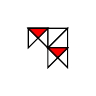
\begin{tikzpicture}[scale=.25]
\draw (0,0) -- (0,1) -- (1,1) -- cycle;
\draw (0,1) -- (1,0) -- (1,1) -- cycle;
\draw (1,1) -- (1,0) -- (2,1) -- cycle;

\draw (1,0) -- (2,0) -- (1,-1) -- cycle;
\draw (2,1) -- (2,0) -- (1,0) -- cycle;

\draw (2,0) -- (2,-1) -- (1,0) -- cycle;

\draw[fill=red] (0,1) -- (0.5,0.5) -- (1,1) --  cycle;
\draw[fill=red] (1,0) -- (1.5,-0.5) -- (2,0) -- cycle;
\end{tikzpicture}
\tiny Calculate $E(P)$
};

\node[block, below of=graphP, yshift=-3cm] (graphP')
{
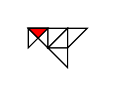
\begin{tikzpicture}[scale=.25]
\draw (0,0) -- (0,1) -- (1,1) -- cycle;
\draw (0,1) -- (1,0) -- (1,1) -- cycle;
\draw (1,1) -- (1,0) -- (2,1) -- cycle;

\draw (2,0) -- (2,1) -- (3,1) -- cycle;
\draw (2,1) -- (2,0) -- (1,0) -- cycle;

\draw (2,0) -- (2,-1) -- (1,0) -- cycle;

\draw[fill=red] (0,1) -- (0.5,0.5) -- (1,1) --  cycle;

\end{tikzpicture}
\tiny Calculate $E(P')$
};

\node[block, below of=graphP, yshift=-0.5cm] (unfoldB)
{
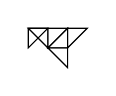
\begin{tikzpicture}[scale=.25]
\draw (0,0) -- (0,1) -- (1,1) -- cycle;
\draw (0,1) -- (1,0) -- (1,1) -- cycle;
\draw (1,1) -- (1,0) -- (2,1) -- cycle;

\draw (2,0) -- (2,1) -- (3,1) -- cycle;
\draw (2,1) -- (2,0) -- (1,0) -- cycle;

\draw (2,0) -- (2,-1) -- (1,0) -- cycle;

\end{tikzpicture}
\tiny Unfold $P'$
};

\node[block, right of=graphP, xshift=3cm, yshift=-2cm] (rand) {Generate $P'$ from $P$; decrease $T$};
\node[block, right of=graphP', xshift=3cm] (better) {$E(P') \leq E(P)$};
\node[block, right of=better, xshift=3cm] (lucky) {$rand(0,1) > 1 - e^{-(T + E(P')/(T_{max})}$};

\node[block, below of=graphP', yshift=-1cm] (over) {$E(P') \leq 0$ or $T \leq 0$};

\node[block, right of=rand, xshift=3cm] (setpP) {Set $P = P'$};

\node[block, below of=over, yshift=-1cm] (finish) {Finish};

\draw[arrow] (graphP') -- (over);

\draw[thick] (better.south) -- (4.5,-9);
\draw[thick] (4.5,-9) -- (12,-9) node[midway, above, sloped] {$true$};
\draw[thick] (12,-9) -- (12,-4.5);
\draw[arrow] (12,-4.5) -- (setpP.east);

\draw[arrow] (better) -- (lucky) node[above, midway, sloped] {$false$};

\draw [arrow] (init) -- (unfoldA);
\draw[arrow] (unfoldA) -- (graphP);
\draw[arrow] (graphP) -| (rand);
\draw[arrow] (rand) -- (unfoldB);

\draw[arrow] (unfoldB) -- (graphP');
\draw[arrow] (setpP) -- (rand);

\draw[thick] (lucky.east) -- (12.0, -7) node[above, midway] {$true$};
\draw[arrow] (lucky) -- (9,-6) -- (4.5,-6) node[midway, above] {$false$} -- (rand);

\draw[arrow] (over.east) -- (2.0,-9.5)  -- (2.0,-7) node[midway, right] {$false$} -- (better.west);

\draw[arrow] (over) -- (finish) node[midway, right] {$true$};
\end{tikzpicture}
\end{document}